\documentclass[11pt,a4paper]{article}
\usepackage[T1]{fontenc}
\usepackage[margin=2.3cm]{geometry}
\usepackage{amsmath,amssymb}
\usepackage{graphicx}
\usepackage[dvipsnames]{xcolor}
\usepackage{enumitem}
\usepackage[colorlinks=true,linkcolor=blue,urlcolor=blue]{hyperref}
\setlength{\parskip}{0.6em}
\setlength{\parindent}{0pt}
\begin{document}

\begin{center}{\LARGE\bfseries openheatpump}\\[0.4em]{\large Size a heat pump and see why it beats a heater, in three sessions.}\\[0.2em]\small PAN IIT OSS explainer \textbullet{} higher secondary to diploma / undergraduate (levels 4-5)\end{center}

\section*{Why this exists}
A resistance heater turns each kilowatt-hour of electricity into one kilowatt-hour of heat. A heat pump moves heat from the outdoor air into the house, so the same electricity can give three or four times as much heat. This explainer shows the mathematics behind that, using only thermodynamic ideas and simple equations, so you can build it yourself.

\section*{The end goal}
Size a heat pump and see why it beats a heater. The end goal is to size a heat pump for a house and see, with your own simulation, why it beats a heater: the COP, the Carnot limit, the house heat loss, the cold-night limits and the yearly cost. It is a simplified educational model, not an installation design.

\section*{How the three sessions build up}
\begin{enumerate}[nosep]
\item \textbf{Session 1: A heat pump moves heat, a heater makes it} (Level 1, conceptual interactive model, 60 min).
\item \textbf{Session 2: COP, the Carnot limit and sizing a heat pump} (Level 2, mathematical engineering model, 75 min).
\item \textbf{Session 3: Simulate a winter hour by hour} (Level 3, simulation and validation, 90 min).
\end{enumerate}

\section{Session 1: A heat pump moves heat, a heater makes it}

\subsection*{A. Real-world problem}
On a cold day a room needs 10 kWh of heat. An electric resistance heater turns every kWh of electricity into exactly 1 kWh of heat, so it uses 10 kWh. A heat pump delivers the same 10 kWh while using only about a quarter of that electricity. That sounds like free energy, so where does the rest of the heat come from, and why does the saving shrink when the weather turns colder? (General education about a simplified model, not an installation design.)

\subsection*{B. Concept and theory}
A resistance heater makes heat: all the electrical energy W becomes heat, so heat out equals W. A heat pump does not make the heat; it moves it from the cold outdoor air into the warm house, much as a pump lifts water uphill, using electricity to do the lifting. The heat delivered is Q\_hot = W + Q\_outdoor, so energy is conserved. The coefficient of performance is COP = Q\_hot / W: the kWh of heat per kWh of electricity. For a heater COP = 1. The lift is the temperature gap between the delivered (supply) temperature and the outdoor temperature; the bigger the gap, the harder the pump works and the lower the COP. The best possible COP for a given gap is T\_hot / (T\_hot - T\_cold) with temperatures in kelvin (K = C + 273.15); real machines reach roughly 40 to 50 percent of it, and we use 0.45 as a typical value.

\begin{itemize}[nosep]
\item W: electrical energy used (kWh)
\item Q\_hot: heat delivered to the house (kWh)
\item Q\_outdoor: heat taken from the outdoor air (kWh)
\item COP: coefficient of performance, Q\_hot / W (no unit)
\item T\_supply, T\_out: temperature of the delivered heat and of the outdoor air (degrees C (kelvin in the formula))
\item eta: fraction of the best possible COP a real machine reaches (typical 0.4 to 0.5) (no unit)
\end{itemize}

\begin{equation*}
Q_{\text{hot}}=W+Q_{\text{outdoor}}\qquad \mathrm{COP}=\frac{Q_{\text{hot}}}{W}\qquad W=\frac{Q_{\text{hot}}}{\mathrm{COP}}
\end{equation*}

\begin{equation*}
\mathrm{COP}_{\text{best}}=\frac{T_{\text{supply}}}{T_{\text{supply}}-T_{\text{out}}},\qquad T[\mathrm{K}]=T[^\circ\mathrm{C}]+273.15
\end{equation*}

\begin{equation*}
\mathrm{COP}\approx \eta\,\frac{T_{\text{supply}}}{T_{\text{supply}}-T_{\text{out}}},\qquad \eta\approx 0.45
\end{equation*}

\begin{center}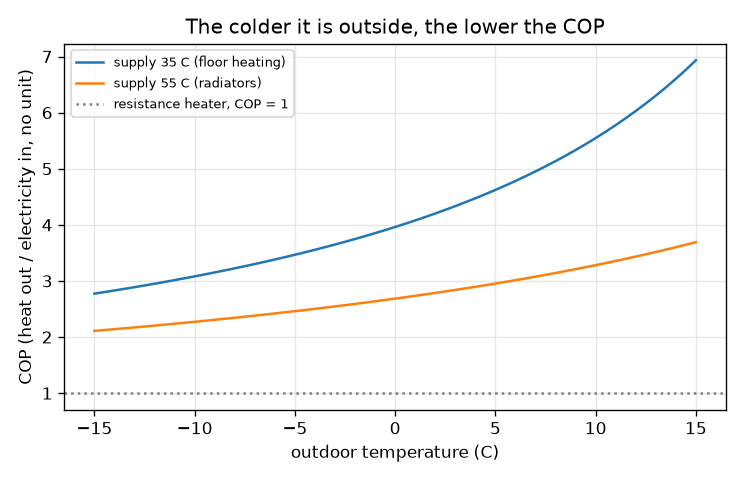
\includegraphics[width=0.85\linewidth]{figures/s01_cop_vs_outdoor.png}\\\small COP against outdoor temperature for 35 C and 55 C supply.\end{center}

\subsection*{E. Worked example}
A house needs 10 kWh of heat. Outdoors it is 0 C and the heat pump delivers heat at 35 C. How much electricity does it use, and how much heat comes from the outdoor air?
\begin{enumerate}[nosep]
\item Convert to kelvin: T\_supply = 35 + 273.15 = 308.15 K; the gap is 35 - 0 = 35 K.
\item Best possible COP = 308.15 / 35 = 8.80. A real machine: COP = 0.45 x 8.80 = 3.96.
\item Electricity W = Q\_hot / COP = 10 / 3.96 = 2.52 kWh.
\item Heat from outdoors = 10 - 2.52 = 7.48 kWh.
\item A resistance heater would need 10.00 kWh, so the heat pump uses about a quarter of the electricity.
\end{enumerate}
\textbf{Answer.} COP 3.96; the heat pump uses 2.52 kWh of electricity and takes 7.48 kWh from the outdoor air; a resistance heater would use 10.00 kWh.

\subsection*{F. Questions}
\begin{enumerate}[nosep]
\item \textbf{Conceptual.} A friend says a heat pump that delivers 4 kWh of heat for 1 kWh of electricity breaks the conservation of energy. Explain why it does not.
\item \textbf{Numerical.} Outdoor 7 C, supply 35 C, eta = 0.45. How much electricity does a heat pump need for 12 kWh of heat, and how much heat comes from outdoors?
\item \textbf{Graph and simulation interpretation.} In the COP graph, at roughly which outdoor temperature does the COP for 35 C supply fall to 3? What about for 55 C supply? What does that tell you about radiators versus floor heating?
\item \textbf{Design and optimisation challenge.} Design: a house needs 10 kWh of heat at 0 C outdoors. Compare a 35 C floor-heating loop with a 55 C radiator loop. Which would you choose and what is the trade-off?
\end{enumerate}

\section{Session 2: COP, the Carnot limit and sizing a heat pump}

\subsection*{A. Real-world problem}
A family wants to heat a 100 square metre house with a heat pump. How big must the machine be so that the house stays at 20 C on a very cold design night of -10 C? How much electricity will it use over a winter compared with a resistance heater, at an illustrative price of 0.25 per kWh? And how cold must it get outside before the heat pump's COP falls too low to be worthwhile? (General education about a simplified model, not an installation design or personal advice.)

\subsection*{B. Concept and theory}
Energy conservation for a heat pump gives Q\_hot = Q\_cold + W. Dividing by W: COP\_heating = COP\_cooling + 1, where COP\_cooling = Q\_cold / W is the figure a fridge cares about. An ideal reversible (Carnot) machine moves heat so that Q\_hot / Q\_cold = T\_hot / T\_cold in kelvin, which gives COP\_heating = T\_hot / (T\_hot - T\_cold). A real COP is a fraction eta of this, typically 0.4 to 0.5, and real machines never reach the huge Carnot values for tiny gaps, so we cap the COP at 8. The house loses heat in proportion to the indoor-outdoor temperature difference: Q\_loss = UA (T\_in - T\_out), where UA is in kW per K. To keep the house at T\_in the heat pump must deliver Q\_loss. Sizing uses a design temperature, a cold outdoor temperature that is reached only rarely. The electricity is Q / COP. Over a heating season we sum 24 h x Q\_loss per day for a heater, and 24 h x Q\_loss / COP for a heat pump, with a COP for each day's temperature.

\begin{itemize}[nosep]
\item Q\_hot, Q\_cold: heat delivered to the house, heat taken from outdoors (kW (power) or kWh (energy))
\item W: electrical work or power (kW or kWh)
\item T\_hot, T\_cold: supply temperature and outdoor temperature in kelvin (K)
\item eta: real COP as a fraction of Carnot (no unit)
\item UA: heat-loss coefficient of the house (area x U-value summed over the envelope) (kW per K)
\item T\_in, T\_out, T\_des: indoor, outdoor and design temperature (degrees C)
\item c: chosen COP floor in the design question (no unit)
\end{itemize}

\begin{equation*}
Q_{\text{hot}}=Q_{\text{cold}}+W\;\Rightarrow\;\mathrm{COP}_h=\mathrm{COP}_c+1
\end{equation*}

\begin{equation*}
\mathrm{COP}_h^{\text{Carnot}}=\frac{T_h}{T_h-T_c}\quad(T\text{ in kelvin}),\qquad \mathrm{COP}\approx\eta\,\mathrm{COP}_h^{\text{Carnot}}
\end{equation*}

\begin{equation*}
Q_{\text{loss}}=UA\,(T_{\text{in}}-T_{\text{out}}),\qquad W=\frac{Q_{\text{loss}}}{\mathrm{COP}}
\end{equation*}

\begin{equation*}
E_{\text{season}}=\sum_{\text{days}}\frac{24\,UA\,(T_{\text{in}}-T_{\text{day}})}{\mathrm{COP}(T_{\text{day}})}
\end{equation*}

\begin{equation*}
T_{\text{cold}}=T_h\left(1-\frac{\eta}{c}\right)\quad\text{(outdoor temperature at which }\mathrm{COP}=c\text{)}
\end{equation*}

\begin{center}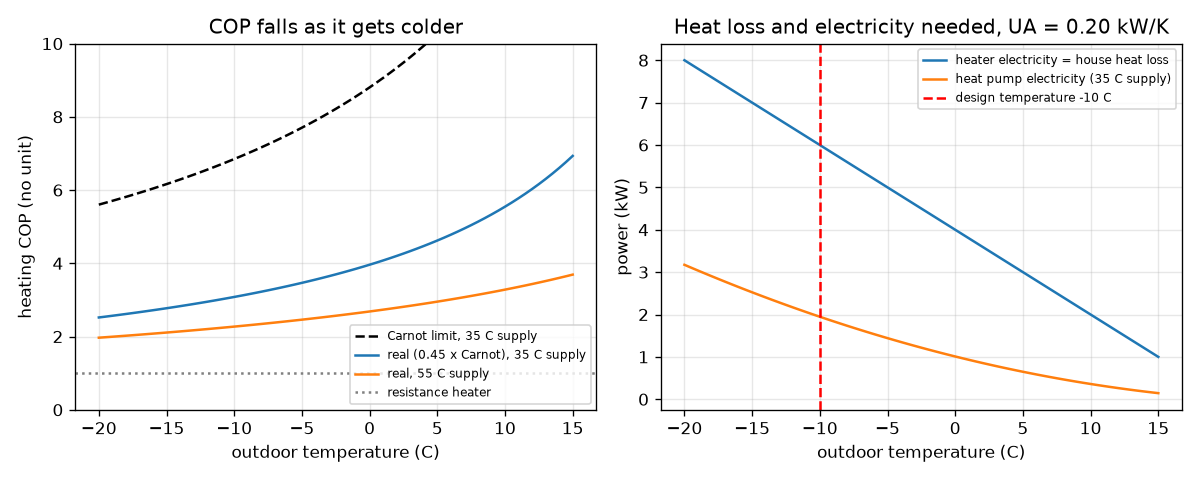
\includegraphics[width=0.85\linewidth]{figures/s02_cop_and_load.png}\\\small Left: Carnot limit and real COP. Right: electric power needed by a heater and a heat pump at UA = 0.20 kW/K.\end{center}

\subsection*{E. Worked example}
A house has UA = 0.20 kW/K and is kept at 20 C. The design temperature is -10 C and the heat pump delivers heat at 35 C with eta = 0.45. Find the design load, the COP and the electric power, then the winter energy and cost for a heater and a heat pump.
\begin{enumerate}[nosep]
\item Design load: Q = 0.20 x (20 - (-10)) = 0.20 x 30 = 6.00 kW. A heat pump must deliver at least 6 kW at -10 C.
\item Carnot COP = 308.15 / (35 - (-10)) = 308.15 / 45 = 6.85; real COP = 0.45 x 6.85 = 3.08.
\item Electric power = 6.00 / 3.08 = 1.95 kW, against 6.00 kW for a resistance heater.
\item Season (151 days with the cosine temperatures): heat needed 12322 kWh. A heater uses 12322 kWh, costing 3080 at 0.25 per kWh.
\item The heat pump uses 2938 kWh (cost 734): a seasonal COP of 12322 / 2938 = 4.19, higher than the design-night COP because most of the season is milder than -10 C.
\end{enumerate}
\textbf{Answer.} Design load 6.00 kW; COP 3.08; electric power 1.95 kW against 6.00 kW; season heat 12322 kWh, heater cost 3080, heat pump 2938 kWh and cost 734 (seasonal COP 4.19).

\subsection*{F. Questions}
\begin{enumerate}[nosep]
\item \textbf{Conceptual.} Why does the heating COP of a heat pump fall as the outdoor air gets colder, even though the machine is unchanged?
\item \textbf{Numerical.} A house has UA = 0.15 kW/K, T\_in = 20 C, design temperature -8 C, supply temperature 45 C and eta = 0.45. Find the design load, the COP at the design temperature and the electric power.
\item \textbf{Graph and simulation interpretation.} In the right-hand graph (power against outdoor temperature) the heater line and the heat pump line both rise as it gets colder. Which rises faster and what does the gap between them mean?
\item \textbf{Design and optimisation challenge.} Design: a radiator system needs 45 C supply. At which outdoor temperature does the COP fall to 2.0 if eta is 0.4, and if it is 0.5? What does that tell you about choosing a machine?
\end{enumerate}

\section{Session 3: Simulate a winter hour by hour}

\subsection*{A. Real-world problem}
Session 2 used daily average temperatures and a house that responds instantly. A real winter has cold nights, a house that takes many hours to cool, a heat pump whose capacity and COP drop in the cold, and a backup heater that rescues it. Can you simulate a whole winter hour by hour, trust the answer, and discover what happens on the coldest night when the heat pump is too small? (General education about a simplified model, not an installation design.)

\subsection*{B. Concept and theory}
The house is one lump with heat capacity C (kWh per K) and loss coefficient UA (kW per K): C dT/dt = Q - UA (T - T\_out). The time constant is tau = C / UA, 20 hours for C = 4.0 and UA = 0.20. If the heat Q is constant during an hour, the exact solution is T\_next = T\_eq + (T - T\_eq) exp(-dt / tau) with T\_eq = T\_out + Q / UA, so the program is stable for any step. The thermostat asks for the heat that would bring the house to the set point at the end of the hour (never negative). The heat pump supplies up to its capacity, which falls with the outdoor temperature (2 percent per kelvin below 7 C, an illustrative figure); a backup resistance heater supplies the rest up to its limit. The COP is eta x Carnot with the supply temperature as a design variable, limited to 8, and multiplied by a defrost factor of 0.9 below 2 C outdoors (an illustrative simple derate). Validation: stored energy change must equal heat supplied minus heat lost, and at constant outdoor temperature the electric power must match UA (T\_set - T\_out) / COP.

\begin{itemize}[nosep]
\item C: heat capacity of the house (kWh per K)
\item UA: heat-loss coefficient (kW per K)
\item tau: time constant C / UA (h)
\item T, T\_out, T\_set: indoor, outdoor and set-point temperature (degrees C)
\item Q\_hp, Q\_bu: heat from the heat pump and from the backup heater (kW)
\item rated: heat pump capacity at 7 C outdoors (kW)
\item T\_supply: temperature at which the heat is delivered (design variable) (degrees C)
\item tariff: price of electricity (money units per kWh)
\end{itemize}

\begin{equation*}
C\,\frac{dT}{dt}=Q-UA\,(T-T_{\text{out}}),\qquad \tau=\frac{C}{UA}
\end{equation*}

\begin{equation*}
T_{n+1}=T_{\text{eq}}+(T_n-T_{\text{eq}})\,e^{-\Delta t/\tau},\qquad T_{\text{eq}}=T_{\text{out}}+\frac{Q}{UA}
\end{equation*}

\begin{equation*}
\mathrm{COP}=\eta\,\frac{T_{\text{sup}}}{T_{\text{sup}}-T_{\text{out}}}\times f_{\text{defrost}},\qquad f_{\text{defrost}}=0.9\ \text{if}\ T_{\text{out}}<2\,^\circ\mathrm{C}
\end{equation*}

\begin{equation*}
C\,(T_{\text{end}}-T_{\text{start}})=\sum (Q_{\text{hp}}+Q_{\text{bu}})\Delta t-\sum UA\,(\bar T-T_{\text{out}})\Delta t
\end{equation*}

\begin{equation*}
W_{\text{steady}}=\frac{UA\,(T_{\text{set}}-T_{\text{out}})}{\mathrm{COP}}
\end{equation*}

\begin{center}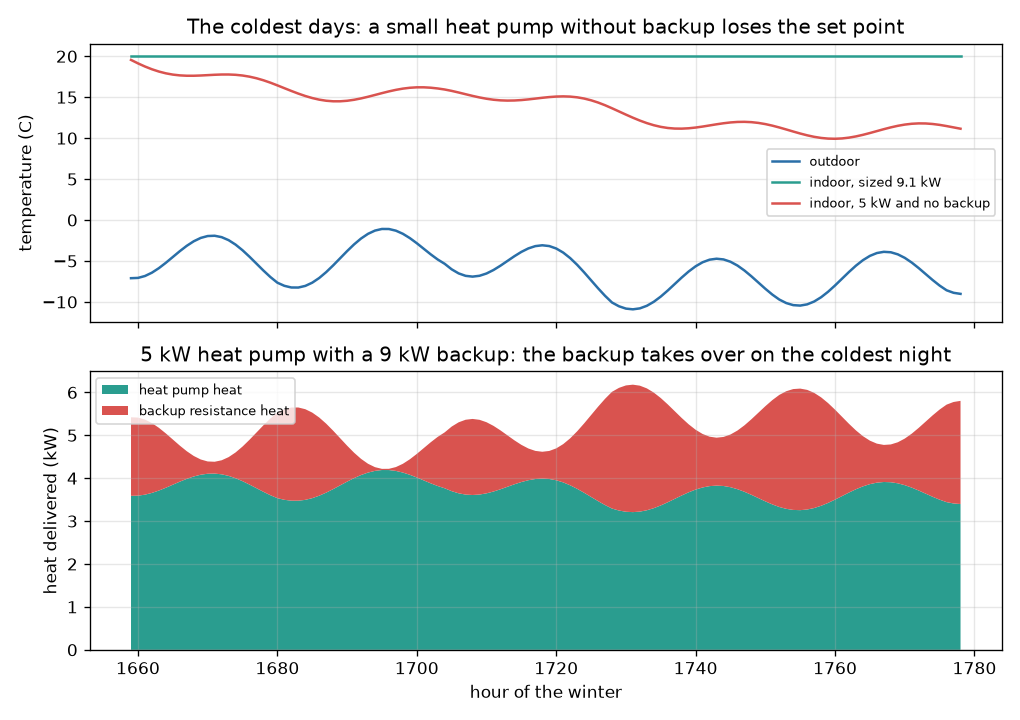
\includegraphics[width=0.85\linewidth]{figures/s03_coldest_nights.png}\\\small The coldest days: a sized heat pump holds 20 C; a small one without backup falls to about 11 C; with backup the extra heat shows in red.\end{center}

\subsection*{E. Worked example}
The house (UA = 0.20 kW/K) is held at 20 C while it is 0 C outdoors for a long time. The supply temperature is 35 C. Find the heat needed, the COP including the defrost derate, and the electric power, and compare with the simulation.
\begin{enumerate}[nosep]
\item Heat needed: Q = 0.20 x (20 - 0) = 4.00 kW.
\item Carnot COP = 308.15 / 35 = 8.80; with eta = 0.45 the COP is 3.962.
\item It is below 2 C outdoors, so the defrost factor 0.9 applies: COP = 3.962 x 0.9 = 3.566.
\item Electric power W = 4.00 / 3.566 = 1.122 kW.
\item The simulation at constant 0 C (300 hours) gives 1.1218 kW in the last hour: they agree.
\item Season (seeded winter, a heat pump rated 9.09 kW sized for -10 C): the heat pump uses 3556 kWh (cost 889, seasonal COP 3.72); a resistance heater uses 13244 kWh (cost 3311), a ratio of 3.7 to 1.
\end{enumerate}
\textbf{Answer.} Heat 4.00 kW, COP 3.566, electric power 1.122 kW, matching the simulation; over the seeded winter the heat pump costs 889 against 3311 for a heater.

\subsection*{F. Questions}
\begin{enumerate}[nosep]
\item \textbf{Conceptual.} On a single very cold night a house with a large heat capacity needs less backup heat than a lightweight house with the same UA. Explain why, and say why it does not help in a long cold spell.
\item \textbf{Numerical.} If the heating fails completely while it is 0 C outdoors, UA = 0.20 kW/K and C = 4.0 kWh/K, how long does the house take to cool from 20 C to 15 C?
\item \textbf{Graph and simulation interpretation.} In the figure, the 5 kW heat pump with backup shows the backup heater switching on in the coldest hours. Estimate the capacity of the 5 kW pump at -11 C and the backup power needed, if the house loss at that temperature is 6.2 kW.
\item \textbf{Design and optimisation challenge.} Design: a poorly insulated house has UA = 0.30 kW/K, 20 C set point, 45 C supply, design temperature -10 C, and a 9 kW backup. Choose a rated capacity: compare the design-temperature size with 10 kW and 8 kW using the seeded winter.
\end{enumerate}

\section{Real-world mini-project}
\textbf{Size a heat pump for a house and estimate its yearly heating cost.} A house has UA = 0.26 kW/K, a 20 C set point and radiators that need a 45 C supply temperature. Its backup heater is 6 kW. Use \texttt{simulate} from Session 3 with the seeded winter and find the smallest rated heat pump capacity (in steps of 0.5 kW) for which the backup heater supplies less than 2 percent of the heat. Compare the winter electricity cost with a resistance heater at 0.25 per kWh. This is general education about a simplified model, not an installation design or personal advice.

\section{The path ahead}
\begin{enumerate}[nosep]
\item \textbf{Session 4: Weather-compensated supply temperature.} A supply temperature that rises linearly as the outdoor temperature falls, limited to 30 to 45 C, used inside the hourly simulation.
\item \textbf{Session 5: On/off thermostat with minimum run time.} A hysteresis thermostat at a sub-hourly step that switches the heat pump fully on or off.
\item \textbf{Session 6: Capital cost and the best size.} A cost model with a price per kW of rated capacity added to the running cost over several winters.
\item \textbf{Session 7: Make the daily model honest.} A correction to the Session 2 daily method (for example a daily-swing and defrost adjustment) tuned against the hourly simulation.
\item \textbf{Session 8: Two-node house and night setback.} A two-capacity house model with a 17 C night set point, integrated with a fourth-order method at a sub-hourly step, drawn like the Target.
\end{enumerate}

\section{Answers and hints}

\subsection*{Session 1}
\begin{enumerate}[nosep]
\item \textbf{Conceptual.} Hint: Write the energy balance with three terms: electricity, outdoor heat and delivered heat. Solution: Energy is conserved because the delivered heat is 1 kWh of electricity plus 3 kWh of heat taken from the outdoor air: 1 + 3 = 4. The pump does not create energy, it moves heat from outside (cold) to inside (warm) and uses the electricity to do so. A heater has no outdoor heat term, so it can give only 1 kWh per kWh.
\item \textbf{Numerical.} Hint: COP = 0.45 x (35 + 273.15) / (35 - 7), then W = Q / COP. Solution: COP = 0.45 x 308.15 / 28 = 4.95. W = 12 / 4.95 = 2.42 kWh. Outdoor heat = 12 - 2.42 = 9.58 kWh. Sanity check: the heat pump uses about a fifth of the 12 kWh a heater would need, and the COP is higher than the 3.96 at 0 C because the gap is smaller.
\item \textbf{Graph and simulation interpretation.} Hint: Find where each curve crosses the level 3. Solve 0.45 x T\_supply / (T\_supply - T\_out) = 3 if you want an exact value. Solution: For 35 C supply the COP is 3 at about -11 C; for 55 C supply it is already 3 at about +6 C. A higher supply temperature means a bigger gap to lift, so the COP is lower at every outdoor temperature: a heat pump with a low-temperature system (floor heating, large radiators) is much more efficient.
\item \textbf{Design and optimisation challenge.} Hint: Compute the COP and the electricity for each supply temperature. Solution: At 35 C: COP 3.96, electricity 2.52 kWh. At 55 C: COP 2.68, electricity 3.72 kWh, about 48 percent more. The low supply temperature is cheaper to run, but it needs a big emitting area (floor loops or oversized radiators) which can cost more to install. Assumption: the same eta of 0.45 for both; real machines also run less efficiently at high supply temperatures.
\end{enumerate}

\subsection*{Session 2}
\begin{enumerate}[nosep]
\item \textbf{Conceptual.} Hint: Look at the Carnot formula and what happens to the denominator T\_hot - T\_cold. Solution: The best possible COP is T\_hot / (T\_hot - T\_cold). A colder outdoor air makes the temperature gap in the denominator bigger, so the COP falls. Physically the machine has to lift heat across a larger temperature difference with the same kind of compressor work. The real COP is a roughly constant fraction of this, so it falls too.
\item \textbf{Numerical.} Hint: Load = UA x (T\_in - T\_des). COP = 0.45 x 318.15 / (45 - (-8)). Solution: Load = 0.15 x 28 = 4.20 kW. COP = 0.45 x 318.15 / 53 = 2.70. Electric power = 4.20 / 2.70 = 1.55 kW. Sanity check: the electric power is about a third of the heat load, and the COP is lower than the 3.08 of the worked example because the supply temperature is higher (45 C rather than 35 C).
\item \textbf{Graph and simulation interpretation.} Hint: Compare the slopes, and read the gap at 0 C and at -10 C. Solution: The heater line rises faster (slope UA = 0.20 kW per K; the heat pump line has a smaller slope because the COP is also falling slowly). The gap is the electric power saved: 2.99 kW at 0 C and 4.05 kW at -10 C, so the heat pump saves most when it is coldest, even though its COP is lowest then.
\item \textbf{Design and optimisation challenge.} Hint: Use T\_cold = T\_hot (1 - eta / c) with kelvin and convert back to Celsius. Solution: T\_hot = 318.15 K. For eta = 0.4: T\_cold = 318.15 x (1 - 0.4 / 2) = 254.52 K = -18.6 C. For eta = 0.5: 318.15 x 0.75 = 238.61 K = -34.5 C. A machine with a better eta keeps the COP above 2 down to much colder weather; the design temperature of the region must be compared with this limit. A COP of 1 (no better than a heater) is not reached until around -100 C in this simple model; in reality, capacity and compressor limits, not the COP, end a heat pump's usefulness.
\end{enumerate}

\subsection*{Session 3}
\begin{enumerate}[nosep]
\item \textbf{Conceptual.} Hint: Think about the stored heat C (T - T\_out) and the time constant tau = C / UA. Solution: A house with a big heat capacity cools slowly (a long time constant), so on one cold night it can lose a degree or two instead of needing extra heating power; the stored heat helps cover the shortfall. In a long cold spell the stored heat is used up, and the heat pump (plus backup) must deliver the full loss UA (T\_in - T\_out) all the time, so the thermal mass delays but does not remove the need for capacity.
\item \textbf{Numerical.} Hint: T = T\_out + (T0 - T\_out) exp(-t / tau). Solve for t with tau = C / UA. Solution: tau = 4.0 / 0.20 = 20 h. 15 = 0 + 20 exp(-t / 20) gives exp(-t / 20) = 0.75, so t = 20 ln(4/3) = 5.75 h. Sanity check: it takes much less than one time constant (20 h) because the drop of 5 K is only a quarter of the 20 K gap.
\item \textbf{Graph and simulation interpretation.} Hint: Capacity = rated x (1 + 0.02 x (T\_out - 7)). Solution: Capacity = 5 x (1 + 0.02 x (-11 - 7)) = 5 x 0.64 = 3.2 kW. The loss is 0.20 x 31 = 6.2 kW, so the backup must give about 3.0 kW. This is why the backup share and the electricity bill jump on the coldest nights: backup heat has a COP of 1 instead of about 3.
\item \textbf{Design and optimisation challenge.} Hint: Design size = load / capacity factor at -10 C, where the factor is 0.66. Then run simulate() for each size and compare cost and backup share. Solution: Load at -10 C is 0.30 x 30 = 9.0 kW, so the rated size is 9.0 / 0.66 = 13.6 kW. Simulation: 13.6 kW costs 1663 with 0.02 percent of the heat from backup; 10 kW costs 1697 (+2 percent) with 1.2 percent backup; 8 kW costs 1811 (+9 percent) with 5.0 percent backup. A smaller machine costs less to buy (capital cost not included here) but uses more backup. A reasonable choice is around 10 kW: the running cost is within 2 percent of the largest machine. Assumptions: illustrative capacity curve and a synthetic winter; a real design needs local weather data and a professional calculation.
\end{enumerate}

\section{How to join}
Read \texttt{CONTRIBUTING.md} in the repository, then pick an issue labelled \texttt{good first issue}. Repository: \url{https://github.com/KrunalPanchal1995/openheatpump}

\end{document}
